%-----------------------------------------------------------------------------%
\chapter{\babTiga}
%-----------------------------------------------------------------------------%

This chapter explains the design and analysis of the \verb|JSONField|
implementation that can be used on all database backends supported by Django.

%-----------------------------------------------------------------------------%
\section{\code{JSONField}}
%-----------------------------------------------------------------------------%

There are two kinds of \verb|JSONField|: the model field and the form field.
The model field is used as an abstraction of the JSON data in the database,
which lets its users manipulate JSON data in the form of Python objects.
The form field is used for accepting JSON data in forms, such as a Django
\verb|ModelForm|.

The model field holds JSON data that can be stored to and retrieved from the
database. In Python, the data is represented in Python's built-in formats:
dictionaries, lists, strings, numbers, booleans, and \verb|None|. When saving
the model, Django executes an SQL \verb|INSERT| or \verb|UPDATE| query to the
database. In order to pass the JSON data in the SQL query, the Python object
has to be serialized into a JSON-encoded string. When retrieving the model
instance, Django executes an SQL \verb|SELECT| query to the database. The data
is retrieved as a JSON-encoded string, which needs to be deserialized, or
decoded, into a Python object.

\begin{figure}
	\centering
    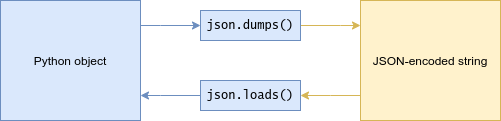
\includegraphics[width=0.66\textwidth]{pics/encodecode.png}
	\caption{The use of the \code{json.dumps()} and \code{json.loads()}
	functions.}
	\label{fig:encodecode}
\end{figure}

To serialize/deserialize Python objects into/from JSON-encoded strings, the
built-in \verb|json| library in Python can be used \cite{python:json}. The
encoding and decoding functionalities are provided through the
\verb|json.dumps()| and \verb|json.loads()| functions, respectively. As shown
by \autoref{fig:encodecode}, the \verb|json.dumps()| function serializes Python
objects into JSON-encoded strings, while the \verb|json.loads()| function
deserializes JSON-encoded strings into Python objects.

The form field utilizes the \verb|json| library for serialization and
deserialization when handling JSON input from the client. If the data being
deserialized is not a valid JSON document, the \verb|json.loads()| function
will raise a \verb|JSONDecodeError|. This error is used by Django to provide
a basic validation functionality by catching the error and raising a
\verb|ValidationError| instead.

\begin{table}
	\centering
	\texttt{
\begin{tabular}{|l|l|}
\hline
\no{\textbf{Python}} & \no{\textbf{JSON}} \\ \hline
dict                 & object    \\ \hline
list \no{or} tuple   & array     \\ \hline
str                  & string    \\ \hline
int\no{,} float\no{,} int\no{- \& }float\no{-derived} Enum\no{s} & number \\ \hline
True                 & true      \\ \hline
False                & false     \\ \hline
None                 & null      \\ \hline
\end{tabular}
}
\captionsource{The data types supported by the built-in \code{JSONEncoder}.}{\cite{python:json}}
\label{table:types-jsonencoder}
\end{table}

\begin{table}
	\centering
	\texttt{
\begin{tabular}{|l|l|}
\hline
\no{\textbf{JSON}} & \no{\textbf{Python}} \\ \hline
object             & dict                 \\ \hline
array              & list                 \\ \hline
string             & str                  \\ \hline
number (int)       & int                  \\ \hline
number (real)      & float                \\ \hline
true               & True                 \\ \hline
false              & False                \\ \hline
null               & None                 \\ \hline
\end{tabular}
}
\captionsource{The data types supported by the built-in \code{JSONDecoder}.}{\cite{python:json}}
\label{table:types-jsondecoder}
\end{table}

By default, the \verb|json.dumps()| function uses the \verb|json.JSONEncoder|
class, while the \verb|json.loads()| function uses the \verb|json.JSONDecoder|
class. These classes support the data types as specified in the JSON
specification and their Python counterparts, as shown by
\autoref{table:types-jsonencoder} and \autoref{table:types-jsondecoder}. To
support other data types and objects, customized \verb|json.JSONEncoder| and
\verb|json.JSONDecoder| subclasses can be used for the functions by supplying
the subclass as the \verb|cls| argument. However, when using a custom decoder,
the deserialization may need to account for the fact that one cannot be certain
of the input type. For example, there is the risk of returning a
\code{datetime} object when decoding a string that just happened to be in the
same format chosen for \code{datetime}s.

\begin{table}
	\centering
	\texttt{
\begin{tabular}{|c|c|c|c|}
\hline
\no{\textbf{Python}}    & \no{\textbf{JSON}} & \no{\textbf{SQL}}            & \no{\textbf{JSON-encoded string}} \\ \hline
'' \no{or} ""  & ""        & ''                  & '""'                     \\ \hline
\{\}           & \{\}      & \no{not applicable} & '\{\}'                   \\ \hline
[]             & []        & \no{not applicable} & '[]'                     \\ \hline
None           & null      & NULL                & 'null'                   \\ \hline
\end{tabular}
}
	\caption{Comparison of empty values and their equivalents in Python, JSON, and SQL.
	The "JSON-encoded string" column shows the Python values after serialization
	with \code{json.dumps()}.}
	\label{table:emptyvalues}
\end{table}

When serializing and deserializing JSON data for the model field, the Python
\verb|None| object, the JSON \verb|null| value, and the SQL \verb|NULL| value
should be taken into consideration. The model field uses JSON-encoded strings
to store JSON values, as there are no SQL equivalents for JSON objects and
arrays. Following the patterns of other values shown by
\autoref{table:emptyvalues}, the \verb|None| object should be stored as the
JSON-encoded \verb|'null'| string in the database. However, according to the
Python DB-API 2.0 specification (which Django follows), the \verb|None| object
is reserved for the SQL \verb|NULL| value for input and output \cite{db-api2}.
Therefore, the model field should skip the serialization and deserialization
for \verb|None| (if it is stored as the top-level value) and let the database
driver store it as SQL \verb|NULL|.\footnote{Storing some data as the top-level
value means that the data is stored directly inside the field, rather than
contained inside a Python dictionary or list.}

In order to store and query the JSON \verb|null| value as the top-level value
of \verb|JSONField|, the \verb|Value| class from the \verb|django.db.models|
module can be utilized. A \verb|Value()| object wraps a literal SQL value to be
used in an SQL expression \cite{django:value}. This literal SQL value is not
processed by Django. In the case of \verb|JSONField|, that means the value is
not passed into the \verb|json.dumps()| function. Therefore, the JSON
\verb|null| value can be stored as a JSON-encoded SQL string literal (i.e.
\verb|Value('null')|). The value will be stored as \verb|'null'|, which is
not \verb|'"null"'| and not \verb|NULL|.

However, when retrieved from the database, both SQL \verb|NULL| and
JSON-encoded \verb|'null'| are represented in Python as \verb|None|. The reason
is that Django processes the \verb|'null'| value using \verb|json.loads()|,
which returns \verb|None|. When \verb|None| is saved as a top-level value in
the database, it is saved as SQL \verb|NULL|. Meanwhile, when querying,
\verb|None| is always interpreted as JSON \verb|null|. To query for SQL
\verb|NULL|, the \verb|isnull| lookup is used.

\listing
{Python}
{A \code{Dog} model with a \code{CharField} for its name and a \code{JSONField}
for additional data.}
{code:dog}
{codes/3-dog.py}

\listing
{Python}
{\code{JSONField} behavior with SQL \code{NULL} and JSON \code{null}.}
{code:null}
{codes/3-null.py}

\autoref{code:null} shows a demonstration of how storing and querying SQL
\verb|NULL| and JSON \verb|null| values work with a \verb|JSONField| defined in
the \verb|Dog| model shown by \autoref{code:dog}. Lines 1 and 2 of
\autoref{code:null} demonstrate storing SQL \verb|NULL|, while lines 3 and 4
demonstrate storing JSON \verb|null| as the top-level value of the field. When
querying as shown by lines 5 and 6, \verb|None| is interpreted as JSON
\verb|null|, hence the query returns the second object. Lines 7 and 8 show that
when querying, using \verb|None| is similar to \verb|Value('null')|. Lines 9
and 10 show that querying for SQL \verb|NULL| can be done using the
\verb|isnull| lookup. Lines 11 and 12 show that JSON \verb|null| is different
from SQL \verb|NULL|, hence the query returns the second object. Lines 13 to 16
show that the \verb|data| field in both objects are represented in Python as
\verb|None|, thus it may be difficult to distinguish between the two.

The behavior of \verb|JSONField| in regards to SQL \verb|NULL| and JSON
\verb|null| may cause confusion, as briefly discussed on the GitHub pull
request shown by
\autoref{fig:nulldiscussion}.\footnote{\url{
	https://github.com/django/django/pull/11452\#discussion\_r335375254}}
The discussion revolved around how Django should deal with JSON \verb|null| as
the top-level value of \verb|JSONField|. It was acknowledged that storing JSON
\verb|null| as the top-level value of \verb|JSONField| is possible by using
\verb|Value|. However, the value will be \verb|None| when retrieved, which
corresponds to SQL \verb|NULL| rather than JSON \verb|null|. As the Django
contributors wrote, the behavior is "tricky and unexpected". While it is
possible to convert the JSON \verb|null| value back into \verb|Value('null')|
when loading it from the database, it is considered as unexpected and "even
less fun". Therefore, to avoid this confusion, Django does not recommend
working with JSON \verb|null| as the top-level value of \verb|JSONField|.

\begin{figure}
	\centering
    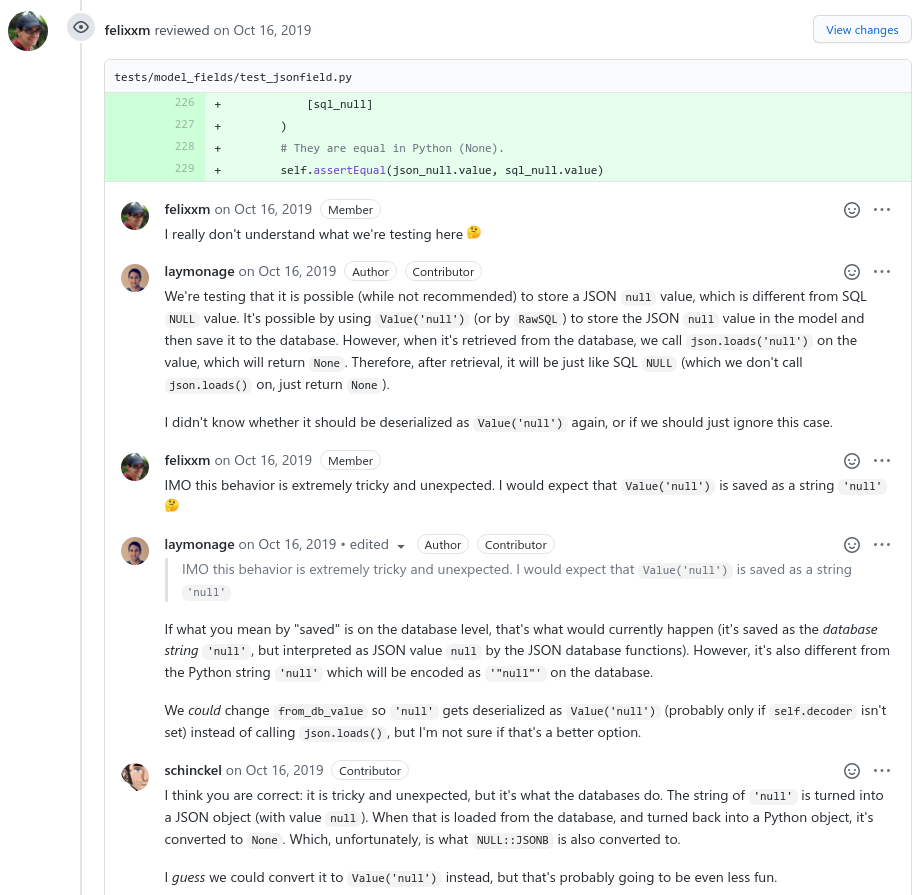
\includegraphics[width=1.0\textwidth]{pics/null_discussion.png}
	\caption{A brief discussion regarding the use of JSON \code{null} as the
	top-level value of a \code{JSONField}.}
	\label{fig:nulldiscussion}
\end{figure}

As with string-based fields such as \verb|CharField| and \verb|TextField|,
Django also recommends avoiding the use of SQL \verb|NULL| on \verb|JSONField|
\cite{django:model_fields}. If the SQL \verb|NULL| is used on a string-based
field, it means that there are two possible values for "no data": \verb|NULL|
and the empty string (\verb|''|). On \verb|JSONField|, it gets more complex:
to represent "no data", there are the empty JSON object (\verb|'{}'|), the
empty JSON array (\verb|'[]'|), the empty JSON string (\verb|'""'|), the JSON
\verb|null| value (\verb|'null'|), and the SQL \verb|NULL|. To avoid
redundancy, it is recommended to set \verb|null=False| (to enforce
database-level \verb|NOT NULL| constraint) on \verb|JSONField| and provide
a suitable default for empty values, such as \verb|default=dict|.

To ensure that the data inserted into the database is valid JSON, the model
field can also define the SQL \verb|CHECK| constraints on the database-level.
On MariaDB and SQLite, the \verb|JSON_VALID()| function can be used as a
\verb|CHECK| constraint \cite{mariadb:json_valid, sqlite:json1}. On Oracle
Database, the \verb|IS JSON| condition can be applied to the table column
\cite{oracle:is_json}. On MySQL and PostgreSQL, the JSON data is automatically
validated when using the \verb|json| data type (or \verb|jsonb| on PostgreSQL)
\cite{postgres:json, mysql:json}. These constraints only validate the syntax of
the JSON data and not the information contained within the data.

This section has covered the design of \verb|JSONField| in terms of storing and
loading JSON data. In addition to storing and loading data, the ORM system in
Django also provides querying capabilities by translating Python method calls
into SQL \verb|SELECT| queries. In order to fully utilize Django's ORM, the
lookups and transforms features of the ORM can be extended to use the JSON
functions provided by the database systems.

%-----------------------------------------------------------------------------%
\section{\code{JSONField} Lookups and Transforms}
%-----------------------------------------------------------------------------%

In Django, lookups and transforms are part of the query expression API. The
API consists of classes that define methods that translate instances of the
classes into SQL expressions. Thus, lookups and transforms can be used to
change how SQL queries are composed by Django, particularly the \verb|WHERE|
clause of \verb|SELECT| queries.

A lookup is a query expression with a left-hand side (\verb|lhs|), right-hand
side (\verb|rhs|), and a \verb|lookup_name| that is used to create a boolean
comparison between \verb|lhs| and \verb|rhs|, such as \verb|lhs < rhs|
\cite{django:lookups}. To use a lookup in a query expression, the notation is
\verb|<lhs>__<lookup_name>=<rhs>|. Since it contains \verb|=<rhs>|, lookups
have to be at the end of a query expression.

Meanwhile, a transform is a query expression that can be used to transform one
field (in an expression) into another field. To use a transform, the notation
is \verb|<expression>__<transform>|. For example, the year transform (e.g.
\verb|date_field__year|) transforms a \verb|DateField| into an
\verb|IntegerField|. As transforms also follow the query expression API, it is
possible to chain multiple transforms in a query expression (e.g.
\verb|<expression>__<transform1>__<transform2>|).

To query JSON data, the previous implementation of \verb|JSONField| included
\verb|JSONField|-specific lookups and transforms. The lookups and transforms
consisted of containment lookups, key existence lookups, and path transforms.
These lookups and transforms were implemented by using JSON operators that are
only available on PostgreSQL. To implement them on other database systems,
those operators need to be substituted with their JSON function equivalents. To
provide a better picture of how lookups and transforms work, they will be
demonstrated using the \verb|Dog| model from \autoref{code:dog} with the
objects created in
\autoref{code:dogobjects}.

\listing
{Python}
{Some \code{Dog} objects created with different JSON data.}
{code:dogobjects}
{codes/3-dogobjects.py}

\listing
{Python}
{A demonstration of the \code{contains} and \code{contained\_by} lookups.}
{code:containment}
{codes/3-containment.py}

The containment lookups consist of the \verb|contains| and \verb|contained_by|
lookups. The \verb|contains| lookup, which normally is used to query for
strings using a case-sensitive substring containment test, is overridden. On
\verb|JSONField|, the lookup is used to query for JSON data using a non-strict
subset containment test. The query will return objects with JSON data that
contains the lookup value as a subset. Meanwhile, the \verb|contained_by|
lookup is the inverse: it looks for objects where the key-value pairs in the
JSON data are a subset of the lookup value.

The \verb|contains| and \verb|contained_by| lookups are demonstrated by
\autoref{code:containment}. In the listing, lines 1 and 2 show that the query
returns objects where the JSON data contains the \verb|{'owner': 'Bob'}|
key-value pair in the top-level. The subset containment test also works with
arrays, as shown by lines 3 and 4. Lines 5 to 7 demonstrate that the query
matches the \verb|<Dog: Meg>| object because its JSON data is a subset of the
lookup value. The query also matches the \verb|<Dog: Fred>| object because an
empty JSON object is a subset of any JSON object, which is also shown by lines
8 and 9.

The containment lookups can be implemented using JSON operators or JSON
functions provided by some of the database systems. On PostgreSQL, the
\verb|contains| and \verb|contained_by| lookups can be implemented using the
\verb|@>| and \verb|<@| operators, respectively \cite{postgres:json_operators}.
On MariaDB and MySQL, both lookups can be implemented using the
\verb|JSON_CONTAINS()| function by switching the target and candidate arguments
for the \verb|contained_by| lookup \cite{mariadb:json_contains,
mysql:json_search}. Unfortunately, SQLite and Oracle Database do not have a
similar function, thus these lookups are left unsupported on both databases.

\listing
{Python}
{A demonstration of the
\code{has\_key}, \code{has\_keys}, and \code{has\_any\_keys} lookups.}
{code:keyexistence}
{codes/3-keyexistence.py}

The key existence lookups consist of the \verb|has_key|, \verb|has_keys|, and
\verb|has_any_keys| lookups. The \verb|has_key| lookup is used to query for
objects where the given key is in the top-level of the JSON data. The
\verb|has_keys| lookup is similar to \verb|has_key|, but it accepts a list of
strings and it is used to query for objects where all of the given keys are
in the top-level of the JSON data. The \verb|has_any_keys| lookup is similar
to \verb|has_keys|, but the objects only need to have at least one of the
given keys in the top-level of the JSON data.

The key existence lookups are demonstrated by \autoref{code:keyexistence}.
Lines 1 and 2 of the listing demonstrate that the \verb|has_key| lookup
returns objects that have the specified key (\verb|'breed'|) in the top-level
of the JSON data. The \verb|has_keys| lookup shown by lines 3 and 4 only
returns objects that have all of the given keys (\verb|'breed'| and
\verb|'favorite_toys'|) in the top-level of the JSON data. As shown by lines 5
and 6, the \verb|has_any_keys| lookup returns objects that have at least one
of the given keys (\verb|'breed'|, \verb|'age'|, or \verb|'favorite_toys'|) in
the top-level of the JSON data.

As with the containment lookups, the key existence lookups can be implemented
using JSON operators or JSON functions on the database systems. On PostgreSQL,
the \verb|has_key|, \verb|has_keys|, and \verb|has_any_keys| lookups can be
implemented using the \code{?}, \code{?\&}, and \code{?|} operators,
respectively \cite{postgres:json_operators}. On MariaDB and MySQL, these
lookups can be implemented using the \verb|JSON_CONTAINS_PATH()| function
\cite{mariadb:json_contains_path, mysql:json_search}. This function accepts
multiple paths as its arguments and there is a \verb|one_or_all| argument that
determines whether the JSON data should contain at least one path or all of the
paths. On SQLite, there is no function that is similar to
\verb|JSON_CONTAINS_PATH()|, but the \verb|JSON_TYPE()| with the
\verb|IS NOT NULL| condition can be used to determine whether a given path
exists \cite{sqlite:json1}. On Oracle Database, a similar functionality can be
obtained using the \verb|JSON_EXISTS()| function \cite{oracle:json_exists}. Both
SQLite and Oracle Database need to chain the function calls with the \verb|AND|
and \verb|OR| operators for the \verb|has_keys| and \verb|has_any_keys|
lookups, respectively.

\listing
{Python}
{A demonstration of the key, index, and path transforms.}
{code:transforms}
{codes/3-transforms.py}

The key, index, and path transforms can be used to query based on a certain
location in the JSON data as shown by \autoref{code:transforms}. To query based
on a given key, the key can be used as the transform name (e.g.
\verb|data__breed|), as shown by lines 1 and 2 of the listing. To query based
on a given path, multiple keys can be chained together using a double
underscore (e.g. \verb|data__owner__name|), as shown by lines 3 and 4. An
integer key, as shown by lines 5 and 6, is interpreted as an array index.

As with other transforms, the \verb|JSONField| transforms can be chained with
the built-in lookups in Django. The built-in lookups consist of the
\verb|exact|, \verb|iexact|, \verb|isnull|, \verb|icontains|,
\verb|startswith|, \verb|istartswith|, \verb|endswith|, \verb|iendswith|,
\verb|regex|, \verb|iregex|, \verb|lt|, \verb|lte|, \verb|gt|, and \verb|gte|
lookups. If there is no lookup specified, the \verb|exact| lookup is used. If
the value for the \verb|exact| lookup is \verb|None|, it will be interpreted as
JSON \verb|null|, as shown by lines 7 and 8. To query for missing keys, the
\verb|isnull| lookup can be used, as shown by lines 9 and 10. Lines 11 and 12
show the transforms chained with the built-in \verb|startswith| lookup, which
matches objects with JSON data at the path \verb|'breed'| that have a value
starting with \verb|'col'|.

The transforms can also be chained with the \verb|JSONField|-specific lookups
described previously. Chaining the transforms with the \verb|contains| lookup
is demonstrated by lines 13 and 14. The lookup matches objects that contain
\verb|{'type': 'ball'}| in any element in the array at the path
\verb|'favorite_toys'| of the JSON data. Chaining the transforms with the
\verb|has_key| lookup is also possible, as shown by lines 15 and 16 where the
query matches objects that have the key \verb|'color'| in the second element of
the array at the \verb|'favorite_toys'| path of the JSON data.

To implement the path transforms, the JSON value specified at the given path
should be extracted. On PostgreSQL, this functionality can be achieved by using
the \verb|->| operator for shallow paths and the \verb|#>| operator for nested
paths \cite{postgres:json_operators}. When the transforms are chained with
lookups that expect a string value on the left-hand side, the \verb|->>| and
\verb|#>>| operators are used instead, so that the value is extracted as
\verb|text| instead of \verb|jsonb|. On MariaDB, MySQL, and SQLite, the
\verb|JSON_EXTRACT()| function can be used \cite{mariadb:json_extract,
mysql:json_search, sqlite:json1}.\footnote{As of version 5.7.13, MySQL also has
\code{->} and \code{->>} operators that work similarly to the \code{\#>} and
\code{\#>>} operators on PostgreSQL. However, MariaDB does not have these
operators, hence the function equivalents are used instead.} When extracting
string values on MariaDB and MySQL, the \verb|JSON_UNQUOTE()| function should be
used to unquote the JSON double quotes \cite{mariadb:json_unquote,
mysql:json_modify}. On Oracle Database, extraction can be done using the
\verb|JSON_VALUE()| function to extract scalar values and the
\verb|JSON_QUERY()| function to extract JSON objects and JSON arrays
\cite{oracle:json_value, oracle:json_query}.

This chapter has described how storing and loading JSON data with
\verb|JSONField| is designed. It has also explained how the
\verb|JSONField|-specific lookups and transforms work, as well as the database
functions that can be used to implement them. In order to implement the design,
some modifications to the Django codebase are required, as explained in the
next chapter.
